% Copyright � 2015 by James Dean Mathias
% All Rights Reserved

\chapter{Mandelbrot Set}\label{appendix:mandelbrot}

The computation and visualization of the Mandelbrot set is used as the basis for demonstrating the techniques presented in this book. Its computation has the features that work well for these topics: computationally intensive, asymmetric complexity, and a visually pleasing result. The purpose of this appendix is to describe its nature and computation for those not already familiar.

\section{Description}

The Mandelbrot set is a fractal\footnote{http://en.wikipedia.org/wiki/Fractal} named after its discoverer Benoit Mandelbrot\footnote{http://en.wikipedia.org/wiki/Benoit\_Mandelbrot}. The Mandelbrot set is visually represented as a two-dimensional image because the numbers in the set lie in the complex number plane. The image shown in Figure \ref{appendix:mandelbrot:overview} shows an example visualization of the set. 

\begin{figure}[H]
	%\begin{mdframed}
	\centering	
	\fbox{
	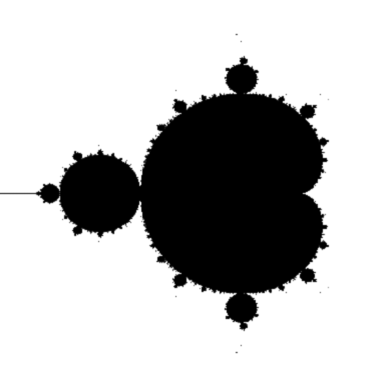
\includegraphics[width=2in, height=2in]{Images/Mandelbrot.png}
	}
	%\end{mdframed}
	\caption{Mandelbrot Overview}
	\label{appendix:mandelbrot:overview}
\end{figure}

The black portion of the image are the points considered to be part of the set, everything else is not. Typically the points outside the set are colored based upon how many iterations it took to determine the point is not part of the Mandelbrot set. In fact, this is the technique used by the demonstration code associated with this book; Section \ref{appendix:mandelbrot:visualization} briefly references how the coloring of the points is determined by the sample code.

\section{Computation}

The Mandelbrot set is given by Equation \ref{appendix:equation:mandelbrot}, where $z_{0} = C$, and $C$ is a complex point in the plane. At any point while iterating this equation, if the distance of $z_{n+1}$ with respect to the origin is greater than 2, then $C$ is not part of the set. Alternatively, if the distance is less than 2 and some maximum number of iterations has been met, then then $C$ is considered to be part of the set. This iterative equation is evaluated for every point over some region of the complex plane.

\begin{equation}
	z_{n+1} = z^{2}_{n} + C
	\label{appendix:equation:mandelbrot}
\end{equation}

The code in \FigureCode \ref{appendix:mandelbrot:computation:code} shows how to compute the number of iterations taken to determine whether or not a point in the complex plane ($C$ = $(x0, y0)$) is part of the Mandelbrot set. The demonstration code associated with this book uses a modified version this listing to perform this same computation.

\begin{code}[caption={Mandelbrot Point Computation}, label=appendix:mandelbrot:computation:code]
uint32_t computePoint(double x0, double y0)
{
  double x = 0;
  double y = 0;
  uint32_t iterations = 0;
  bool done = false;

  while (!done)
  {
    double tempX = x * x - y * y + x0;
    y = 2.0 * x * y + y0;
    x = tempX;

    double distance = x * x + y * y;
    // Saving sqrt by comparing vs 4
    if (distance > 4.0 || iterations >= MAX_ITERATIONS)
    {
      done = true;
    }
    iterations++;
  }

  return iterations;
}
\end{code}

The parameters \texttt{x0} and \texttt{y0} are the coordinates of a point in the complex number place. This point is $C$ of the equation, which means it is also $z_{0}$; the initial value for the iterative computation. Remember, the mathematics are in terms of numbers on the complex plane. With this in mind, the first two lines that follow the \texttt{while (!done)} statement are the computation for $z_{n+1}$ in the iterative sequence. The next value of \texttt{y} is already updated, the third line then is to capture the updated value of \texttt{x}. With the next value of $z$ computed, it is time to test the distance of it from the center of the complex number plane. The square of the distance is computed and stored in \texttt{distance}. The reason for storing the square of the distance is to save the (expensive) computation of taking a square root. With the square of the distance the comparison is made against the value of 4, rather than 2; with 4 being the square of 2. At the same time, the test for the maximum allowed iterations is made. If either of their conditions is true, the iterative computation is terminated and the final \texttt{iterations} result is returned.

What makes the Mandelbrot set a great example for this book is that the number of iterations for each point varies from one point to the next. This results in the computational complexity varying over the image, especially when lines, or groups of lines, are used as the basic comptuational building block. Having this computational asymmetry over the image works well to demonstrate the computational load balancing that occurs through the application of the techniques described in this book.

\section{Visualization}\label{appendix:mandelbrot:visualization}

To create a visualization of the Mandelbrot set, all points within some complex region must be computed. Given that the entire set, by definition, must be within a distance of 2 from the origin, it only makes sense to define a plane that lies in the range of $(-2, -2)$ and $(2, 2)$. This complex region must be mapped onto a rectangular region of image pixels, for example a 1000 x 1000 pixel sized image. Given this mapping, each pixel is then associated with a complex number. This complex number is then fed into a function that computes the number of iterations for which the equation was evaluated. Finally, the number of iterations is used to determine the color for that pixel.

There are many different ways to decide the color for a Mandelbort visualization. The simplest is to select from two colors, for example black or white, depending upon whether or not the pixel is part of the set. Another is to use color to indicate the number of iterations used to calculate the pixel set membership. In order to to this a range of colors is defined and evenly divided based upon the the maximum possible iterations, then a color is selected based upon the iteration count. Another is to create a histogram that tracks how many times (the frequency) each iteration count was used. Then associate a color with each bucket in the histogram and color.  Another is to use a continuous, or smooth, coloring technique that eliminates the \textit{banding} associated with many of the other coloring algorithms. The examples in this book all use a smooth coloring technique.

For those interested in more detail about the Mandelbrot set and the various coloring algorithms, please visit  \href{http://en.wikipedia.org/wiki/Mandelbrot\_set}{http://en.wikipedia.org/wiki/Mandelbrot\_set}.
